\subsection{Change Management}

\indent 

\noindent \textbf{Change Management (CM)}: the \textbf{structured approach to guiding individuals, teams, and organizations from their current state to a desired future state}. It focuses not just on what is changing (new systems, processes, or structures), but how people adopt and embrace that change.

\bigskip

\noindent Why does it matter in IT?

In IT projects, success isn’t just about delivering the technology on time and on budget (that’s project management). True success comes when the end-users adopt the new system or process, integrate it into their daily work, and deliver business value. Research shows that projects with excellent change management are 6x more likely to meet or exceed objectives than those with poor CM.

\subsubsection{Difference between Project and Change management}

\begin{table}[h]
\centering
\begin{tabular}{|c|l|l|}
\hline
\textbf{Aspect}          & \multicolumn{1}{c|}{\textbf{Project Management}}                                                                              & \multicolumn{1}{c|}{\textbf{Change Management}}                                                                                           \\ \hline
\textbf{Core Focus}      & \begin{tabular}[c]{@{}l@{}}Ensures the technical side \\ of change is delivered - \\ scope, time, cost, quality.\end{tabular} & \begin{tabular}[c]{@{}l@{}}Ensures the people side \\ of change is managed \\ – adoption, engagement, \\ mindset, behaviors.\end{tabular} \\ \hline
\textbf{Goal}            & Deliver the solution.                                                                                                         & Deliver the adoption of the solution.                                                                                                     \\ \hline
\textbf{Scope}           & \begin{tabular}[c]{@{}l@{}}Planning, scheduling, budgeting, \\ risk management, resources, \\ deliverables.\end{tabular}      & \begin{tabular}[c]{@{}l@{}}Communication, training, \\ stakeholder management, \\ overcoming resistance.\end{tabular}                     \\ \hline
\textbf{Success measure} & \begin{tabular}[c]{@{}l@{}}Did we deliver on time, \\ on budget, to scope?\end{tabular}                                       & \begin{tabular}[c]{@{}l@{}}Are people using it? \\ Are they confident, \\ competent, and committed?\end{tabular}                          \\ \hline
\end{tabular}
\end{table}

\subsection{Change}

\subsubsection{The 3 states of change}

\begin{itemize}
    \item Current state: where the organisation is today (comfort zone, existing processes).
    \item Transition state: the “messy middle” where old ways are being abandoned but new ways aren’t yet stable.
    \item Future state: the desired new reality where the change is fully adopted and embedded.
\end{itemize}

\subsubsection{The Kubler-Ross Change Curve}

\indent 

People go through predictable stages when faced with change. Productivity and morale usually \textbf{drop before they improve}. Change managers anticipate this dip and support people through it.

\begin{figure}[h]
    \centering
    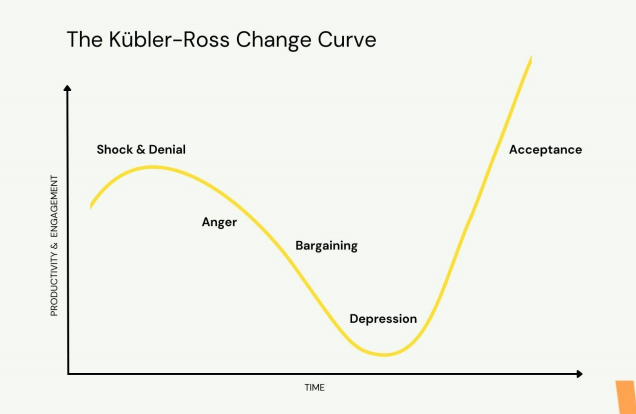
\includegraphics[width=0.5\linewidth]{figures/Week 7/KR Curve.png}
\end{figure}

\bigskip

\noindent\textbf{Stages of the Change curve}:

\begin{itemize}
    \item Shock and Denial
    \begin{itemize}
        \item In IT: “The old system works fine. This project will never happen.”
        \item CM Focus: Provide clear information about why the change is happening
    \end{itemize}
    \item Anger
    \begin{itemize}
        \item - In IT: “Why are we forced to use this? Management doesn’t understand our work!”
        \item CM Focus: Encourage listening and empathy; give people a safe channel to voice concerns
    \end{itemize}
    \item Bargaining
    \begin{itemize}
        \item In IT: “Can’t we keep using the old CRM for some tasks? Maybe run both in parallel?”
        \item CM Focus: Provide clarity on non-negotiables and offer small flexibilities where possible.
    \end{itemize}
    \item Depression
    \begin{itemize}
        \item In IT: “This is too hard. Productivity is dropping. I can’t keep up.”
        \item CM Focus: Offer training, coaching, and peer support. Share quick wins to rebuild confidence.
    \end{itemize}
    \item Acceptance
    \begin{itemize}
        \item In IT: “Okay, I can see the benefits now. This system actually makes my job easier.”
        \item CM Focus: Reinforce positive behaviours, celebrate successes, embed the change into culture.
    \end{itemize}
\end{itemize}

\subsubsection{Key implications for IT Projects}

\indent 

Transition state is the riskiest $\xrightarrow{}$ confusion, mistakes, drop in productivity.

Change managers need to provide communication, training, and support to help people move through the curve.

Success depends on moving the majority from resistance to commitment efficiently.

\subsubsection{Psychology of Change}

\noindent Why does psychology matter in IT Change?

Even the best-designed IT systems fail \textbf{if people resist} or refuse to adopt them.

Change creates \textbf{uncertainty} $\xrightarrow{}$ humans are wired to seek stability, routine, and control.

Psychology helps us understand \textbf{why people resist} and \textbf{how to support them}.

\bigskip

\noindent \textbf{Common Psychological Responses}

\begin{itemize}
    \item \textbf{Fear of the Unknown}: “What will this mean for my job?”
    \item \textbf{Loss Aversion}: People value what they already have more than what they might gain.
    \item \textbf{Cognitive Dissonance}: Conflict between old habits and new expectations.
    \item \textbf{Status Quo Bias}: Preference to “keep things as they are.”
    \item \textbf{Social Proof}: People adopt changes faster when they see peers/colleagues doing so.
\end{itemize}

\bigskip

\noindent\textbf{Theories and perspectives}

\begin{itemize}
    \item Change agents must be conscious of both a sender's mentality and the receiver's orientation.
    \item Employee resistance is the norm, not the exception. Expect some to never support the change.
    \item Visible and active sponsorship is not only desirable but necessary for success.
    \item Value systems have a direct impact on how employees react to change.
    \item The size of change determines how much and what kind of change management is needed.
    \item The "right" answer is not enough to successfully implement change.
    \item Employees go through the change process in stages and go through these stages as individuals.
\end{itemize}

\noindent\textbf{Supporting Psychology of Change}:

\begin{itemize}
    \item \textbf{Empathy}: listen and acknowledge concerns.
    \item \textbf{Communication}: explain the “why,” not just the “what.”
    \item \textbf{Involvement}: give people a voice in shaping the change.
    \item \textbf{Training \& Coaching}: reduce anxiety by building competence.
    \item \textbf{Reinforcement \& Recognition}: reward early adopters, celebrate progress
\end{itemize}

\subsubsection{Managing Change Effectively}

\indent

Everyone has a different pace of adapting to change. This can be seen through the Diffusion of Innovation Theory:

\begin{itemize}
    \item \textbf{Early adopters}: curious, motivated by innovation.
    \item \textbf{Majority}: wait until they see proof of benefits.
    \item \textbf{Laggards}: fear loss, need strong support to shift.
\end{itemize}

\bigskip

\noindent\textbf{Core principles of Effective Change Management}

\begin{itemize}
    \item \textbf{Clarity of Purpose}: Communicate the why (business case, benefits).
    \item \textbf{Leadership Commitment}: Senior leaders must actively champion the change.
    \item \textbf{Stakeholder Engagement}: Involve the right people early, listen to concerns.
    \item \textbf{Structured Process}: Follow a proven framework (ADKAR, Kotter, etc.).
    \item \textbf{Continuous Support}: Training, coaching, feedback channels throughout the transition.
\end{itemize}

\bigskip

\noindent  Key activities in IT Projects:

\begin{itemize}
    \item Build awareness and desire: Explain why change is necessary
    \item Develop capability: Provide training, job aids, and coaching
    \item Reinforce adoption: Recognise early adopters, collect feedback, and adjust quickly
\end{itemize}

\subsubsection{Practical Strategies for IT Change}

\begin{itemize}
    \item \textbf{Communication Plan}:
    \begin{itemize}
        \item Tailored messaging for executives, managers, end-users.
        \item Multi-channel: town halls, FAQs, videos, Slack/Teams updates.
    \end{itemize}
    \item \textbf{Stakeholder Mapping \& Resistance Management}:
    \begin{itemize}
        \item Identify “high influence, low support” individuals early.
        \item Convert them into champions or neutralize risks.
    \end{itemize}
    \item \textbf{Quick Wins \& Iterative Delivery}:
    \begin{itemize}
        \item Agile-style pilots $\xrightarrow{}$ demonstrate success quickly.
        \item Use feedback loops to refine adoption strategies.
    \end{itemize}
    \item \textbf{Change Agents Network}:
    \begin{itemize}
        \item Identify respected staff in each department.
        \item Train them to support peers → peer influence accelerates adoption.
    \end{itemize}
\end{itemize}

\subsubsection{Change and Business \& IT outcomes}

\indent

\noindent Why is change and outcomes related?

\begin{itemize}
    \item IT projects succeed only when \textbf{people adopt the change}.
    \item Without adoption → business value is never realized (new system unused, shadow IT emerges, money wasted).
    \item Effective OCM ensures the investment in technology translates into results.
\end{itemize}

\bigskip 

\noindent On successful change management, a few business outcomes could be:

\begin{itemize}
    \item Higher Productivity: Faster processes, reduced errors, smoother workflows.
    \item Customer Satisfaction: Improved service delivery, quicker response times.
    \item Employee Engagement: Staff feel supported and involved → reduced turnover.
    \item Innovation Readiness: Organization builds resilience for future changes.
\end{itemize}

\bigskip On successful change management, a few IT outcomes could be:

\begin{itemize}
    \item Adoption Rates: Percentage of users actively engaging with the new system.
    \item System Utilization: Depth of features being used vs. basic functions only.
    \item Process Compliance: Are new workflows followed, or do people revert to old ways?
    \item Governance Alignment: Supports ITIL Change Enablement and compliance standards.
\end{itemize}

\subsection{OCM Models and Frameworks}

\subsubsection{McKinsey's 7s Model}

\indent 

It is a holistic framework to analyze and align an organization during change. It focuses on \textbf{seven interdependent elements}, divided into hard and soft factors.

\begin{itemize}
    \item Hard S’s (easier to identify \& manage):
    \begin{itemize}
        \item \textbf{Strategy}: the plan to build competitive advantage.
        \item \textbf{Structure}: organizational hierarchy, reporting lines.
        \item \textbf{Systems}: processes, workflows, and IT systems.
    \end{itemize}
    \item Soft S’s (harder to define, but critical for success):
    \begin{itemize}
        \item \textbf{Shared Values}: the organization’s core beliefs and culture (the central point).
        \item \textbf{Skills}: capabilities and competencies of staff.
        \item \textbf{Style}: leadership style and management approach.
        \item \textbf{Staff}: people, roles, and talent management.
    \end{itemize}
\end{itemize}

\bigskip

\noindent\textbf{Benefits of this model}

\begin{itemize}
    \item Encourages \textbf{holistic thinking} (not just focusing on systems or strategy).
    \item Identifies \textbf{misalignments} that block change (e.g., great strategy but no skills to execute).
    \item Useful for diagnosing why change is stalling.
    \item Can act as a \textbf{checklist} during IT and business transformation.
\end{itemize}

\bigskip

\noindent \textbf{When to use?}

\begin{itemize}
    \item During \textbf{major IT implementations} (ERP, HRMS, CRM, etc.) to ensure people, processes, and systems align.
    \item For \textbf{organizational restructuring}.
    \item To \textbf{assess readiness} for change.
    \item To \textbf{troubleshoot failing projects} by identifying gaps.
\end{itemize}

\subsubsection{ADKAR Model}

\indent 

Focuses on guiding \textbf{individuals through change}, step by step. The acronym stands for the \textbf{five building blocks} of successful change.

\begin{itemize}
    \item \textbf{A – Awareness}
    \begin{itemize}
        \item People understand why the change is happening.
        \item “Why this change? Why now?”
    \end{itemize}
    \item \textbf{D – Desire}
    \begin{itemize}
        \item Individuals are motivated to support the change.
        \item Overcomes resistance by showing personal and organizational benefits.
    \end{itemize}
    \item \textbf{K – Knowledge}
    \begin{itemize}
        \item Training and communication provide people with how to change.
        \item Skills, tools, and understanding are built.
    \end{itemize}
    \item \textbf{A – Ability}
    \begin{itemize}
        \item People apply knowledge and perform in the new way.
        \item Requires practice, coaching, and support.
    \end{itemize}
    \item \textbf{R – Reinforcement}
    \begin{itemize}
        \item Sustains change through recognition, rewards, and performance tracking.
        \item Prevents “slipping back” into old habits.
    \end{itemize}
\end{itemize}

\bigskip

\noindent\textbf{Benefits of the model}

\begin{itemize}
    \item \textbf{Simple, people-centered framework} (easy to teach and apply).
    \item Breaks down change into \textbf{manageable, actionable steps}.
    \item Highlights that \textbf{change happens at the individual level first}.
    \item Helps managers \textbf{diagnose resistance} (e.g., if adoption is failing, is it Awareness or Ability that’s missing?).
\end{itemize}

\bigskip

\noindent\textbf{When to use?}

\begin{itemize}
    \item IT rollouts where \textbf{end-user adoption} is key (e.g., CRM, ERP, HRMS).
    \item Agile projects requiring \textbf{continuous adoption}.
    \item Situations with \textbf{high resistance} where people need structured support.
    \item \textbf{Training and enablement programs} linked to IT change.
\end{itemize}

\subsubsection{Kotter's 8 step change model}

\indent 

A \textbf{top-down approach} to managing organizational change.

Focuses on creating momentum and embedding change into culture.

\noindent\textbf{The 8 steps}:

\step Create a sense of urgency: Show why change is needed now.

\step Build a Guiding Coalition: Form a strong team of leaders and influencers to drive change.

\step Develop a vision and strategy: Provide a clear direction for the change and how it benefits the organization.

\step Communicate the change vision: Share the message widely and consistently. Use multiple channels (emails, town halls, team meetings).

\step Empower Employees for action: Remove barriers and provide resources.

\step Generate short term wins: Show quick, visible results to keep motivation high.

\step Consolidate gains and produce more change: Use early successes to drive further change. Don’t declare victory too soon.

\step Anchor new approaches in the culture: Embed change into policies, processes, and values.

\bigskip

\noindent\textbf{Benefits of the model}:

\begin{itemize}
    \item Provides a \textbf{structured roadmap} for large-scale change.
    \item Focuses on \textbf{leadership and communication}.
    \item Ensures \textbf{momentum is sustained} beyond early wins.
    \item Particularly strong for \textbf{strategic IT transformations}.
\end{itemize}

\bigskip

\noindent\textbf{When to use?}

\begin{itemize}
    \item Large, organization-wide IT changes (e.g., digital transformation, ERP rollout).
    \item When culture change is essential for adoption.
    \item In hierarchical organizations where \textbf{leadership sponsorship} is critical.
\end{itemize}

\subsection{Questions}

\subsubsection{End of Lecture Questions}

\begin{itemize}
    \item What is the difference between project management and change management? Why do IT projects need both?
    \item How does change management contribute to business and IT outcomes? Give one business outcome and one IT outcome.
    \item Compare the McKinsey 7S, ADKAR, and Kotter’s 8-step models. In which scenarios would each be most effective?
    \item How does OCM support IT governance and frameworks such as ITIL Change Enablement?
\end{itemize}

\subsubsection{Case Study}

\indent 

Alpha Manufacturing is a mid-sized company that decides to implement a new Enterprise Resource Planning (ERP) system to integrate finance, supply chain, and HR.

The Project Management team focuses on budget, schedule, and vendor 
coordination.

The Change Management team is tasked with employee adoption and 
training.

\noindent Challenges emerging:

\begin{itemize}
    \item Many employees are skeptical, saying the old systems “work fine.”
    \item Line managers feel excluded from decision-making.
    \item Training sessions are poorly attended.
    \item A pilot rollout showed low adoption: employees continue using spreadsheets.
    \item The CIO is under pressure to show ROI within 12 months.
\end{itemize}

\bigskip

\noindent\textbf{Questions}:

\begin{itemize}
    \item At which stage(s) of the change curve do Alpha’s employees seem to be?
    \item What psychological factors might be causing resistance to the ERP system?
    \item Which change management model (McKinsey 7S, ADKAR, or Kotter’s 8-step) would you apply to this situation? Why?
    \item What 2–3 practical steps could the Change Management team take to increase adoption and reduce resistance?
\end{itemize}